%%%% utfpr-poster.tex, 2019/12/01
%%%% Copyright (C) 2018-2019 Luiz E. M. Lima (luizeduardomlima@gmail.com)
%%
%% This work may be distributed and/or modified under the conditions of the
%% LaTeX Project Public License, either version 1.3 of this license or (at your
%% option) any later version.
%% The latest version of this license is in
%%   http://www.latex-project.org/lppl.txt
%% and version 1.3 or later is part of all distributions of LaTeX version
%% 2005/12/01 or later.
%%
%% This work has the LPPL maintenance status `maintained'.
%%
%% The Current Maintainer of this work is Luiz E. M. Lima.
%%
%% This work consists of the files utfpr-poster.sty and utfpr-poster.tex.
%%
%% A brief description of this work is in readme.txt.

%% Detecção e aviso sobre comandos obsoletos
% \RequirePackage[l2tabu, orthodox]{nag}

%% Classe de documento e opções
\documentclass[%% Opções: [>] passada para pacotes
  final,%% Em oposição à de rascunho (draft) [>]
  english,%% Idioma secundário (penúltimo) [>]
  english,%% Idioma primário (último) [>]
]{beamer}

%% Pacotes utilizados
\usepackage[%% Opções: [>] passada para beamerposter
  Times   = false,%% Fontes Times (roman) e Arial (sans serif): true ou false
  BibURLs = true,%% Links de URLs nas referências: true ou false
  ABNTNum = none,%% Estilo numérico ABNT: none (AUTOR, ANO), dflt (1) e brkt [1]
  size    = custom,%% Tamanho de papel: a0, a1, a2, a3, a4 e custom [>]
  width   = 90,%% Largura de papel em centímetros (custom) [>]
  height  = 120,%% Altura de papel em centímetros (custom) [>]
  scale   = 1.5,%% Escala de fontes [>]
]{utfpr-poster}
\usepackage{hyperref}

%\renewcommand{\figurename}{Figure}

%% Arquivo de referências
\addbibresource{utfpr-poster.bib}

%% Informações do documento
%%%% Título
\title{%
  REAL-TIME HAND GESTURE CONTROL %
  \\OF A ROBOTIC ARM WITH PROGRAMMABLE MOTION MEMORY%
}
%%%% Assunto
\subject{ICINCO}
%%%% Autor(es)
\author{%
  Daniel Giraldi Michels\inst{1}%
  \orcidlinkicon{0009-0005-5037-8815}%
  \and Davi Giraldi Michels\inst{1}%
  \orcidlinkicon{0009-0004-9627-0431}%
  \and Lucas Alexandre Zick\inst{2}\inst{3}%
  \orcidlinkicon{0009-0001-8645-9781}%
  \and Dieisson Martinelli\inst{1}%
  \orcidlinkicon{0000-0001-7589-1942}%
  \and André Schneider de Oliveira\inst{1}%
  \orcidlinkicon{0000-0002-8295-366X}%
  \and and Vivian Cremer Kalempa\inst{1}%
  \orcidlinkicon{0000-0001-9733-7352}%
}
%%%% Instituição(ões) e e-mail(s)
\institute{%
  \affil[1]{\utfprname, Curitiba, Paraná, Brasil}%
  \and\affil[2]{Department of Information Systems, Universidade do Estado de Santa Catarina (UDESC), São Bento do Sul, Brazil}%
  \and\email[]{daniel.michels@edu.udesc.br}%
  \sep\email[]{davi.michels@edu.udesc.br}%
  \sep\email[]{zick@alunos.utfpr.edu.br}%
  \sep\email[]{dmartinelli@alunos.utfpr.edu.br}%
  \sep\email[]{andreoliveira@utfpr.edu.br}%
  \sep\email[]{vivian.kalempa@udesc.br}%
}
%%%% Data: comente para gerar a data atual
\date{}

%% Início do documento
\begin{document}

\begin{frame}[t, fragile = singleslide]

\begin{columns}[t, onlytextwidth]%% Início do cabeçalho
%
\begin{column}{0.1\textwidth}
\begin{flushleft}

\includegraphics[width = \columnwidth]{./Logos/logo_ICINCO_2025}%% Logomarca superior-esquerdo
\vspace*{0.5\baselineskip}

\includegraphics[width = \columnwidth]{./Logos/logo_INSTICC_2}%% Logomarca inferior-esquerdo
\end{flushleft}
\end{column}
%
\begin{column}{0.8\textwidth}
\titlepage%
\end{column}
%
\begin{column}{0.1\textwidth}
\begin{flushright}

\includegraphics[width = \columnwidth]{./Logos/logo_utfpr}%% Logomarca superior-direito
\vspace*{0.5\baselineskip}

\includegraphics[width = \columnwidth]{./Logos/logo_planalto_norte.png}%% Logomarca inferior-direito
%\vspace*{0.5\baselineskip}
%
\includegraphics[width = \columnwidth]{./Logos/logo_IPB_2}%% Logomarca
% \vspace*{0.5\baselineskip}
% \meclogo%% Logomarca do Ministério da Educação
% \vspace*{0.5\baselineskip}
% \govlogo%% Logomarca do Governo Federal
\end{flushright}
\end{column}
%
\end{columns}%% Fim do cabeçalho

\begin{columns}[t, onlytextwidth]
%
\begin{column}{0.49\textwidth}
%
\begin{block}{INTRODUCTION}
Current teleoperation methods often rely on physical devices like joysticks or data gloves \cite{zick2024teleoperation,martinelli2020human}, but are frequently limited by high cost, complexity, and a lack of intuitive control, hindering their widespread adoption \cite{moniruzzaman2022teleoperation}.

To overcome these shortcomings, this paper proposes an innovative control method for articulated robotic arms. The proposed method utilizes real-time recognition of the user's hand position and movements using a single camera, as can be seen in Figure \ref{fig:uso_do_sistema}.

\vspace{-0.15cm}
\begin{figure}[!htb]
    \centering
    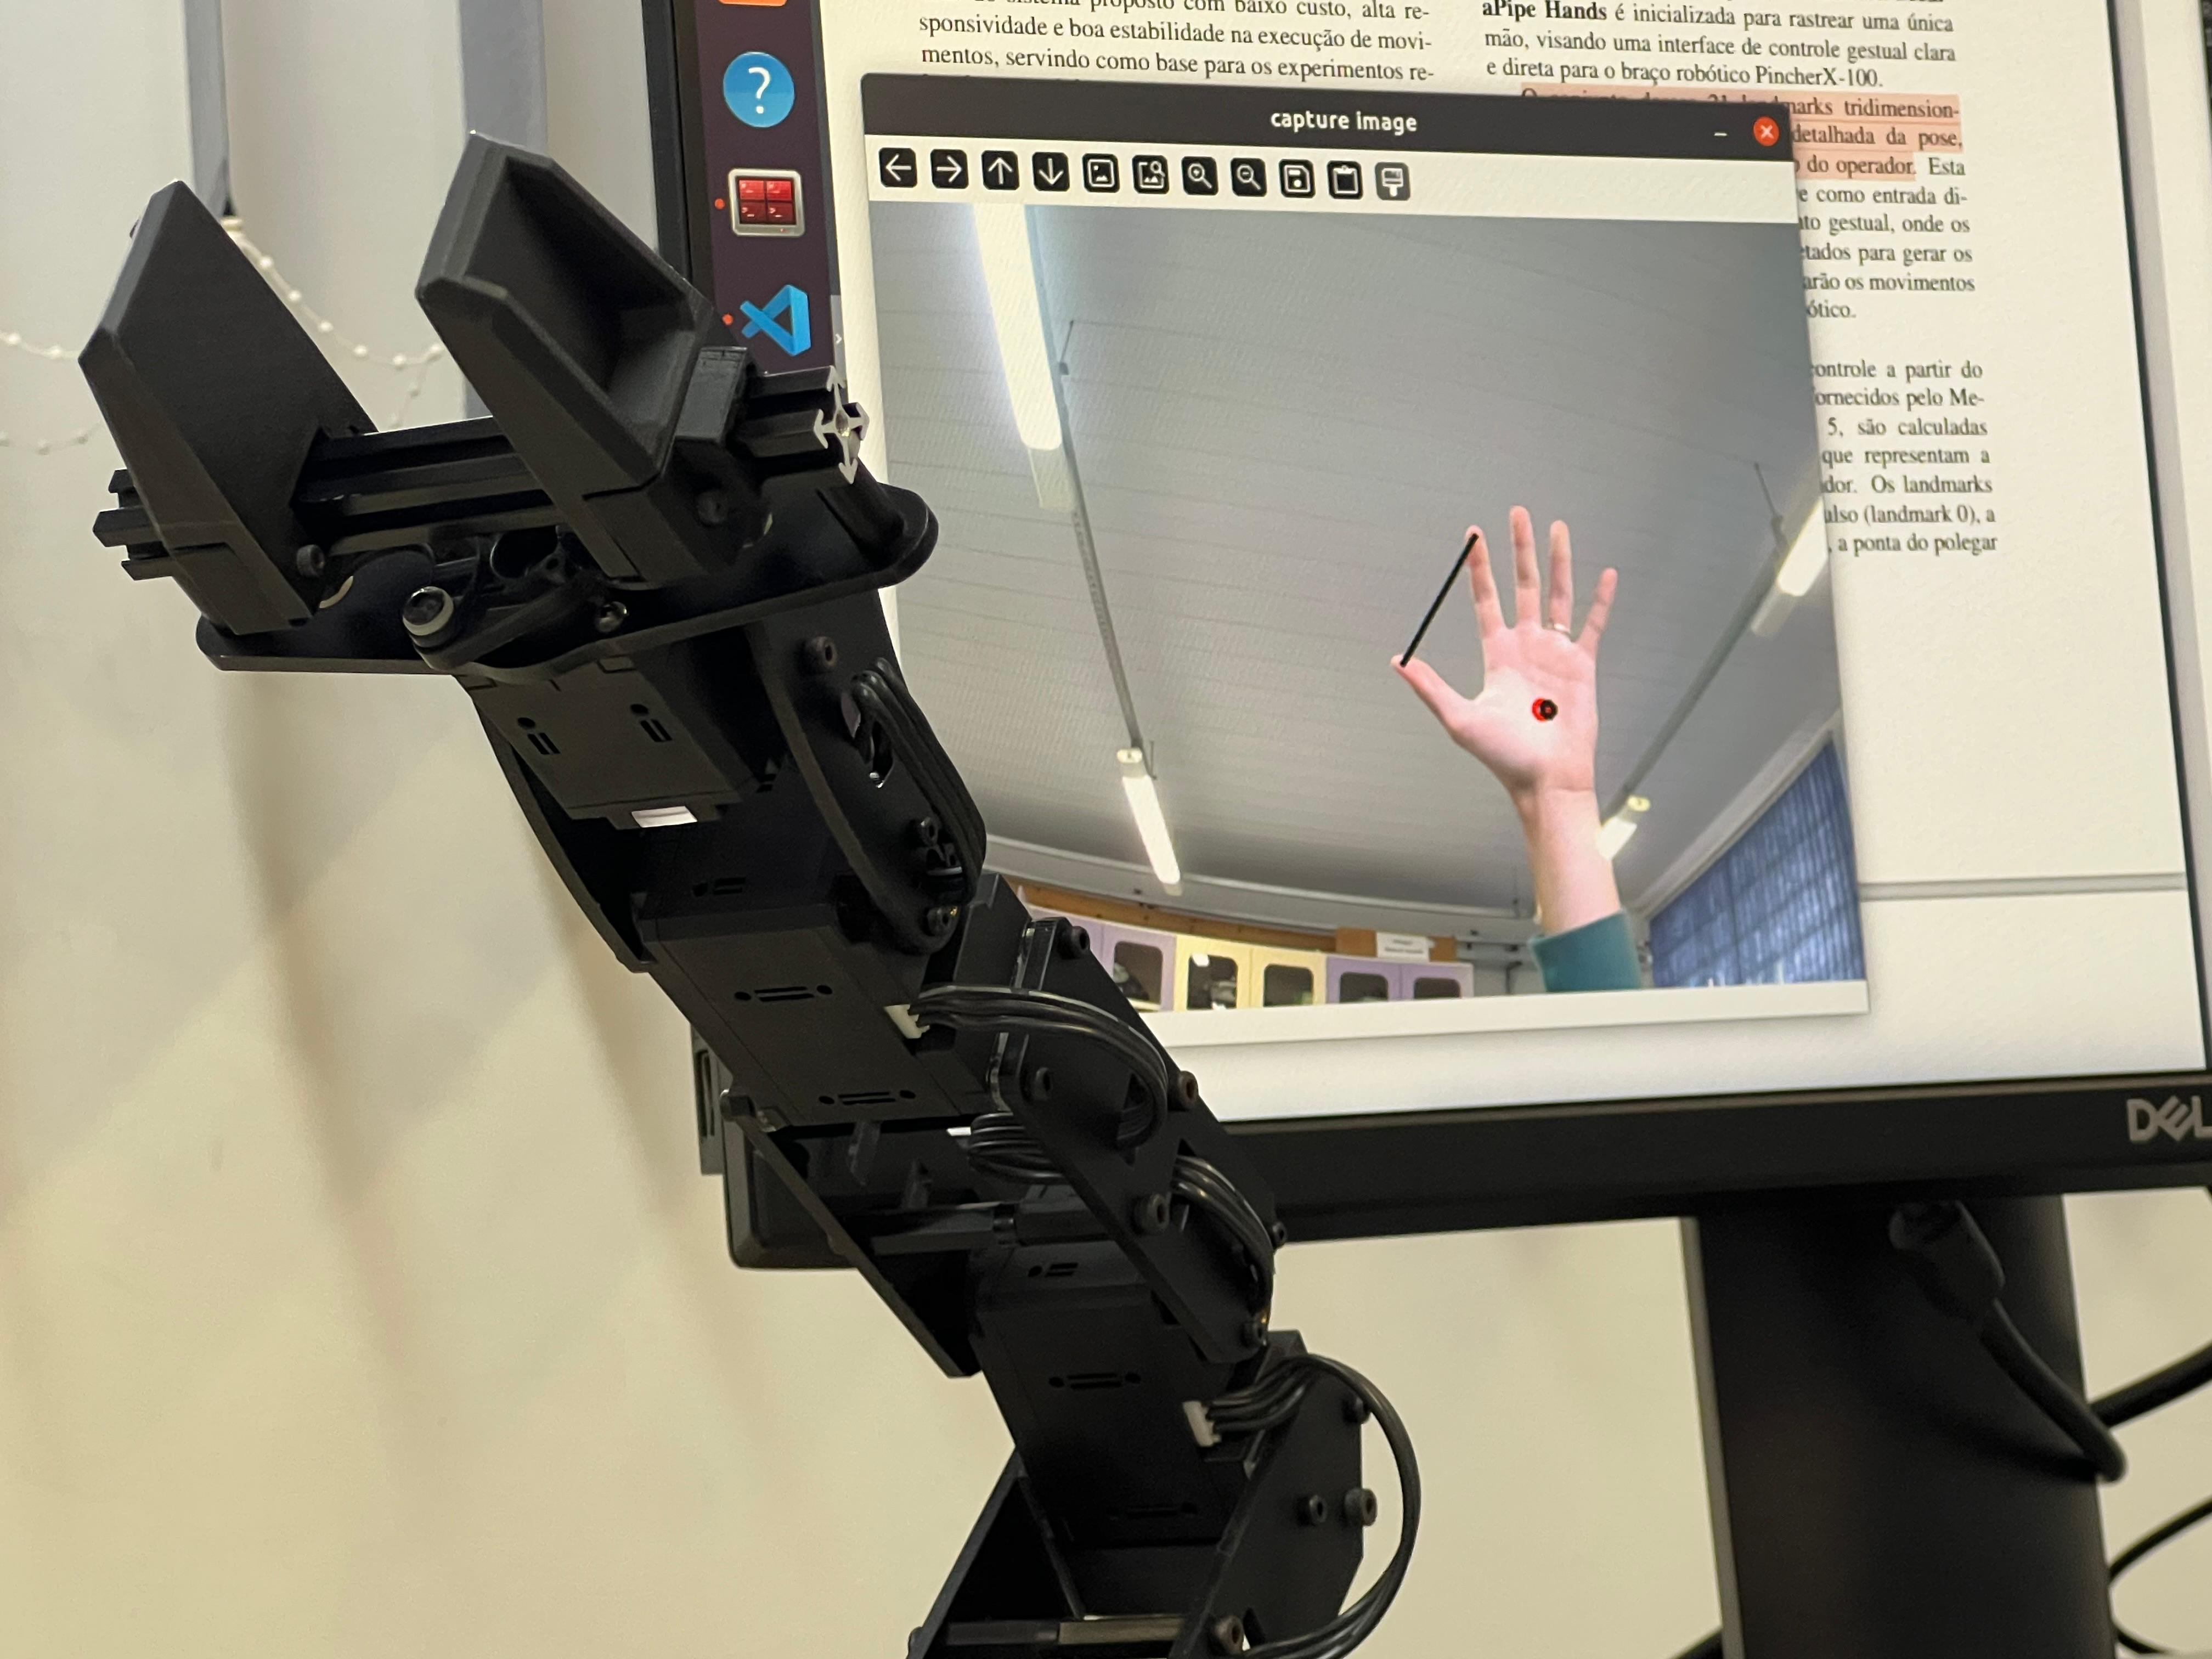
\includegraphics[scale=0.15]{Figuras/hand_and_robot.jpeg}
    \caption{System usage.}
    \label{fig:uso_do_sistema}
\end{figure}

A distinctive feature of our system is its ability to store and reproduce movement sequences, which greatly simplifies the automation of repetitive tasks by enabling "Programming by Demonstration".

\end{block}
% 
% \begin{block}{RELATED WORK}

% Existing research in robotic teleoperation has explored advanced interfaces, including multi-robot control systems, deep learning for motion recognition, and immersive virtual reality environments \cite{zick2024teleoperation, martinelli2020human, franzluebbers2019remote}. While powerful, these approaches often require specialized hardware or complex implementations. In contrast, this work presents a low-cost and accessible alternative by leveraging a single RGB camera with the MediaPipe library. Our key contribution is the integration of a 'Programming by Demonstration' feature, enabling intuitive task automation without additional sensors.

% \end{block}


\begin{block}{EXPERIMENTAL VALIDATION}
To evaluate the system's effectiveness, precision, and repeatability, we designed a "pick and place" test, simulating a common industrial task. The experiment required the robotic arm to pick up a 4 cm cube from a platform elevated by 13 cm and place it on a ground-level surface approximately 30 cm away. An operator first demonstrated the task once using hand gestures, which the system recorded. Subsequently, the system was commanded to autonomously execute the stored movement for 50 consecutive cycles, during which the number of successful attempts and the time per cycle were logged for analysis. A demonstration video of the test is available at:

\begin{figure}[htbp]
    \centering
    % Certifique-se que o nome do arquivo 'grafico_tempos.png' corresponde ao seu arquivo de imagem
    
\includegraphics[width=.2\columnwidth]{Figuras/QR_Code.png} 
    \caption{A demonstration video of pick and place test.}
    \label{fig:qrcode}
\end{figure}

\end{block}

\begin{block}{CONCLUSION}
This work validated a viable and effective solution for intuitive robotic programming, successfully bridging the gap between human intention and robotic execution. The high success rate (98\%) and consistency in cycle time (0.0126s standard deviation) empirically confirm the system's robustness, precision, and repeatability. We demonstrate that a low-cost, camera-based approach can significantly reduce the complexity of traditional robotic programming, making automation more accessible. Future work will focus on implementing conditional logic based on gestures and abstracting the software to ensure portability across different robot models.

\end{block}

%
%
%
%
\end{column}
%
%%%%%%%%%%%%%%%%%%%%%%%%%%%%%%%%%%%%%%%%%%%%%%%%%%%%%%%%%%%%%%%%%%%%%%%%%%%%%%%%%%%%%%%%%%%%%%%%%%%%%%%%%%%%%%%%%%%%%%%%%%%%%%%%%%
\begin{column}{.49\textwidth}
% 
\begin{block}{PROPOSED STRATEGY}

Our system's architecture comprises three modules: Gesture Capture, Robot Command Mapping, and Trajectory Recording. The high-level control logic was implemented in Python, using an Interbotix PincherX-100 robotic arm controlled via the Robot Operating System (ROS) \cite{ros}. Real-time gesture capture is achieved with a standard camera and the MediaPipe library \cite{mediapipe}, which tracks 21 3D hand landmarks. The hand's position is mapped to the robot's base and elbow joints, while a calculated depth variable controls the shoulder's reach. The gripper is actuated by the distance between the thumb and index fingertips. This intuitive control, facilitated by OpenCV \cite{opencv_library} for image processing and the \texttt{interbotix\_xs\_modules} library for arm communication, is enhanced by a programming module that allows the operator to Record (\texttt{'R'}), Play (\texttt{'P'}), and Loop (\texttt{'L'}) a demonstrated trajectory.

\end{block}
%
\begin{block}{RESULTS}
The system demonstrated high robustness and effectiveness, achieving a 98\% success rate, with 49 out of 50 trials completed successfully presented in Table\ref{tab:pick_place_results}. The quantitative analysis also confirmed the excellent precision and repeatability of the method. The mean cycle time was 13.35 seconds, with a very low standard deviation of only 0.0126 seconds. The execution time remained remarkably stable across all 50 repetitions, indicating no performance degradation over time and confirming the system's reliability for repetitive tasks.
%The experiments’ evolution, as the system’s scalability was increased to observe possible variations in the system’s behavior, the position of the swarm throughout the experiment, and the potential field associated with the swarm’s initial position are illustrated by Figure 3. An other important result is presented in Figure 4 by the yellow% plane performed by the central robot for gas source localization. %Table \ref{tab:principais_resultados_exp2} contains the average values of the obtained results.


\begin{table}[h]
    \caption{"Pick and Place" Test Results (50 Repetitions)}
    \label{tab:pick_place_results}\centering
    \resizebox{0.4\linewidth}{!}{%
    \begin{tabular}{|l|r|}
        \hline
        \textbf{Metric} & \textbf{Value} \\
        \hline
        Total Trials & 50 \\
        Successful Trials & 49 \\
        Failures & 1 \\
        Success Rate & 98\% \\
        Mean Cycle Time (s) & 13.35 \\
        Time Std. Deviation (s) & 0.0126 \\
        \hline
    \end{tabular}}
\end{table}


% \begin{figure}[htbp]
%     \centering
%     % Certifique-se que o nome do arquivo 'grafico_tempos.png' corresponde ao seu arquivo de imagem
%     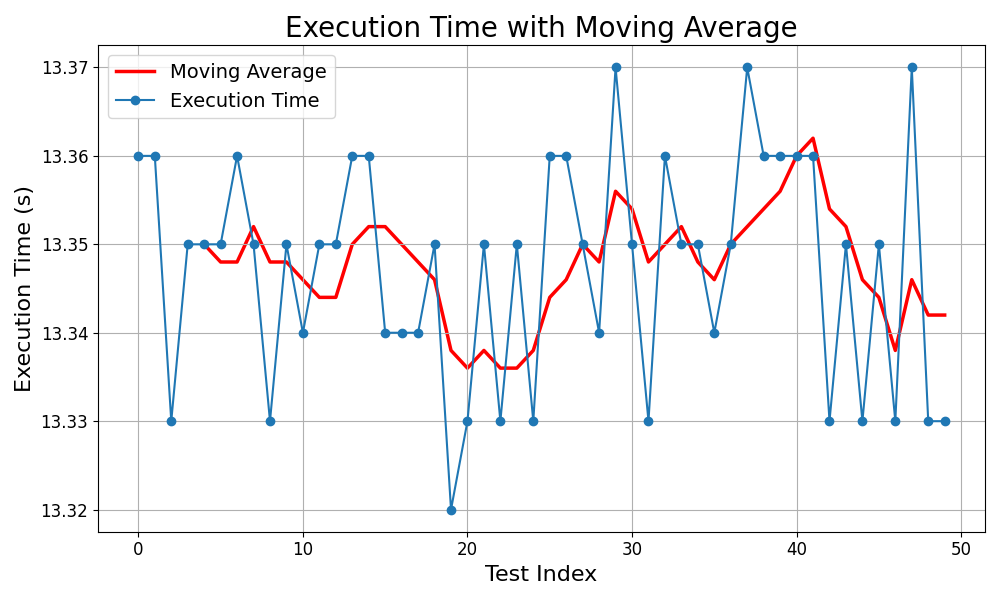
\includegraphics[width=.7\columnwidth]{Figuras/validation_graphic.png} 
%     \caption{Execution time per cycle for 50 trials, with the moving average in red.}
%     \label{fig:execution_times}
% \end{figure}

\end{block}
%
\begin{block}{REFERENCES}
  \printbibliography[heading = none]
\end{block}
%
\begin{block}{ACKNOWLEDGEMENTS}
\footnotesize%
The funding organizations, for the support received for the development of this work and participation in this event:
\vfill%

\includegraphics[height = 20mm]{./Logos/apoio-capes}
\hspace*{5mm}

\includegraphics[height = 20mm]{./Logos/apoio-cnpq}
\hspace*{5mm}

\includegraphics[height = 20mm]{./Logos/apoio-fa-gov-pr}
\hspace*{5mm}

\includegraphics[height = 20mm]{./Logos/fa}
\hspace*{5mm}

\includegraphics[height = 20mm]{./Logos/seti}
\hspace*{5mm}

\includegraphics[height = 20mm]{./Logos/utfpr}
\hspace*{5mm}

\includegraphics[height = 20mm]{./Logos/napi_robotica.png}
\hspace*{5mm}

\includegraphics[height = 20mm]{./Logos/logo_UDESC_vertical.png}
\end{block}
%

\end{column}
\end{columns}

\vspace*{\stretch{1000}}

\begin{columns}[b]
%
\begin{column}{0.49\textwidth}
\respnotice[Declaration of Responsibility]{the author(s) are solely responsible for the information contained in this document.}
\end{column}
%
\begin{column}{0.49\textwidth}
\begin{flushright}

\includegraphics[height = 20mm]{./Logos/utfpr-110anos}%% Logomarca comemorativa da UTFPR (110 anos)
\hspace*{5mm}

\includegraphics[height = 20mm]{./Logos/utfpr}%% Logomarca da UTFPR-PG
% \hspace*{5mm}
% \meclogobottom%% Logomarca do Ministério da Educação
% \hspace*{5mm}
% \govlogobottom%% Logomarca do Governo Federal
\end{flushright}
\end{column}
%
\end{columns}

\vspace*{\baselineskip}

\end{frame}

%% Fim do documento
\end{document}
